\subsection{Tail load extraction and the structural mass loop}
\label{sec:tail-structural-loop}

The aerodynamic enlargement was followed by a structural-demand calculation,
rather than an assumption that a larger tail could retain adequate stiffness
at unchanged mass. AVL strip and surface forces were extracted again at the
frozen original, enlarged-tail and added-point-mass equilibria. Integrated
strip lift was checked against the separately printed surface coefficient;
left and right half-panel loads were also checked for symmetry. Table~\ref{tab:tail-beam-demand}
reports the vertical-bending screen, using each half-panel as a clamped beam
starting at $|y|=0.55$ m. Downward self-weight was included under an assumed
uniform panel mass. This is not a verified representation of the actual
tail attachment or a gust/maneuver load envelope.

\begin{table}[htbp]\centering\small
\caption{Conditional demands for one tail half at the evaluated equilibrium.}
\label{tab:tail-beam-demand}
\begin{tabular}{lrrr}\toprule
Case & Upward lift (N) & Root moment magnitude (N m) & $EI$ for 10 mm (N m$^2$)\\\midrule
Original V15 & -107.053 & 168.297 & 21,630\\
Enlarged tail & -75.469 & 293.888 & 117,435\\
Enlarged tail plus 2 kg & -65.727 & 274.402 & 109,843\\\bottomrule
\end{tabular}\end{table}

Although the enlarged tail carries less downward aerodynamic force at its
new equilibrium, its longer span and increased self-weight raise the bending
and stiffness demands. For a strip load $F_i$ at distance $a_i$ from a clamped
root, its contribution to tip displacement multiplied by constant $EI$ is
$F_i a_i^2(3l-a_i)/6$. This kernel was checked against both an end point load
and the uniform-load beam solution. The reported 10 mm displacement is an
exploratory parameter, not a demonstrated clearance or serviceability limit;
5 and 20 mm were retained as sensitivity cases.

A subsequent 210-section hollow-rectangle trade used the USDA clear-wood
mean for Sitka spruce at 12\% moisture, $E=10.8$ GPa, and specific gravity
0.40 \cite{ref46}. Density was calculated as $0.40(1000)(1.12)=448$ kg/m$^3$.
These modern property data are evaluator inputs, not knowledge supplied to the
historically constrained models. The clear-wood strength values are not
aircraft design allowables: grade, grain slope, defects, moisture, joint
efficiency and variability remain important. The equivalent boxes assume
effective load transfer between their walls; fabrication and historical
availability of such a construction were not established.

With original tail mass retained and beam self-weight added, the least-mass
section meeting the illustrative 20 mm displacement screen within the stated
grid had a 160 by 160 mm envelope and 3 mm walls. The two beams add 6.794 kg;
their first-order predicted tip displacement is 17.29 mm under the original
enlarged-tail load distribution plus their own weight. Re-trimming the
light-pilot, empty-fuel case with that distributed added mass on the coarse
mesh changes the surface-model margin to $-0.221\%$. This candidate is therefore
not accepted. The calculation is deliberately additive: no unsubstantiated
credit was taken for an unspecified original spar. It does not prove that
all possible cantilever tails fail; it rejects this particular mass-and-section
experiment, whose fit and connections also remain unresolved.

\paragraph{A tension-braced alternative.}
Figure~\ref{fig:braced-tail-concept} defines a separate researcher concept.
Two 120 by 100 mm equivalent wood boxes with 4 mm walls occupy the spanwise
hinge/spar line. A central 40 mm square mast extends 0.35 m above and below
that line. Four 4 mm wires join its ends to the outer tail stations.
The wire horizontal span is 4.575 m from the centerline mast, whereas the
beam's exposed length is 4.025 m from its root: these two dimensions must not
be interchanged. The mast is intended to rotate with the all-moving tail;
that mechanism has not yet been reconciled with the fuselage cross-members,
bearing arrangement and control horn.

\begin{figure}[htbp]\centering
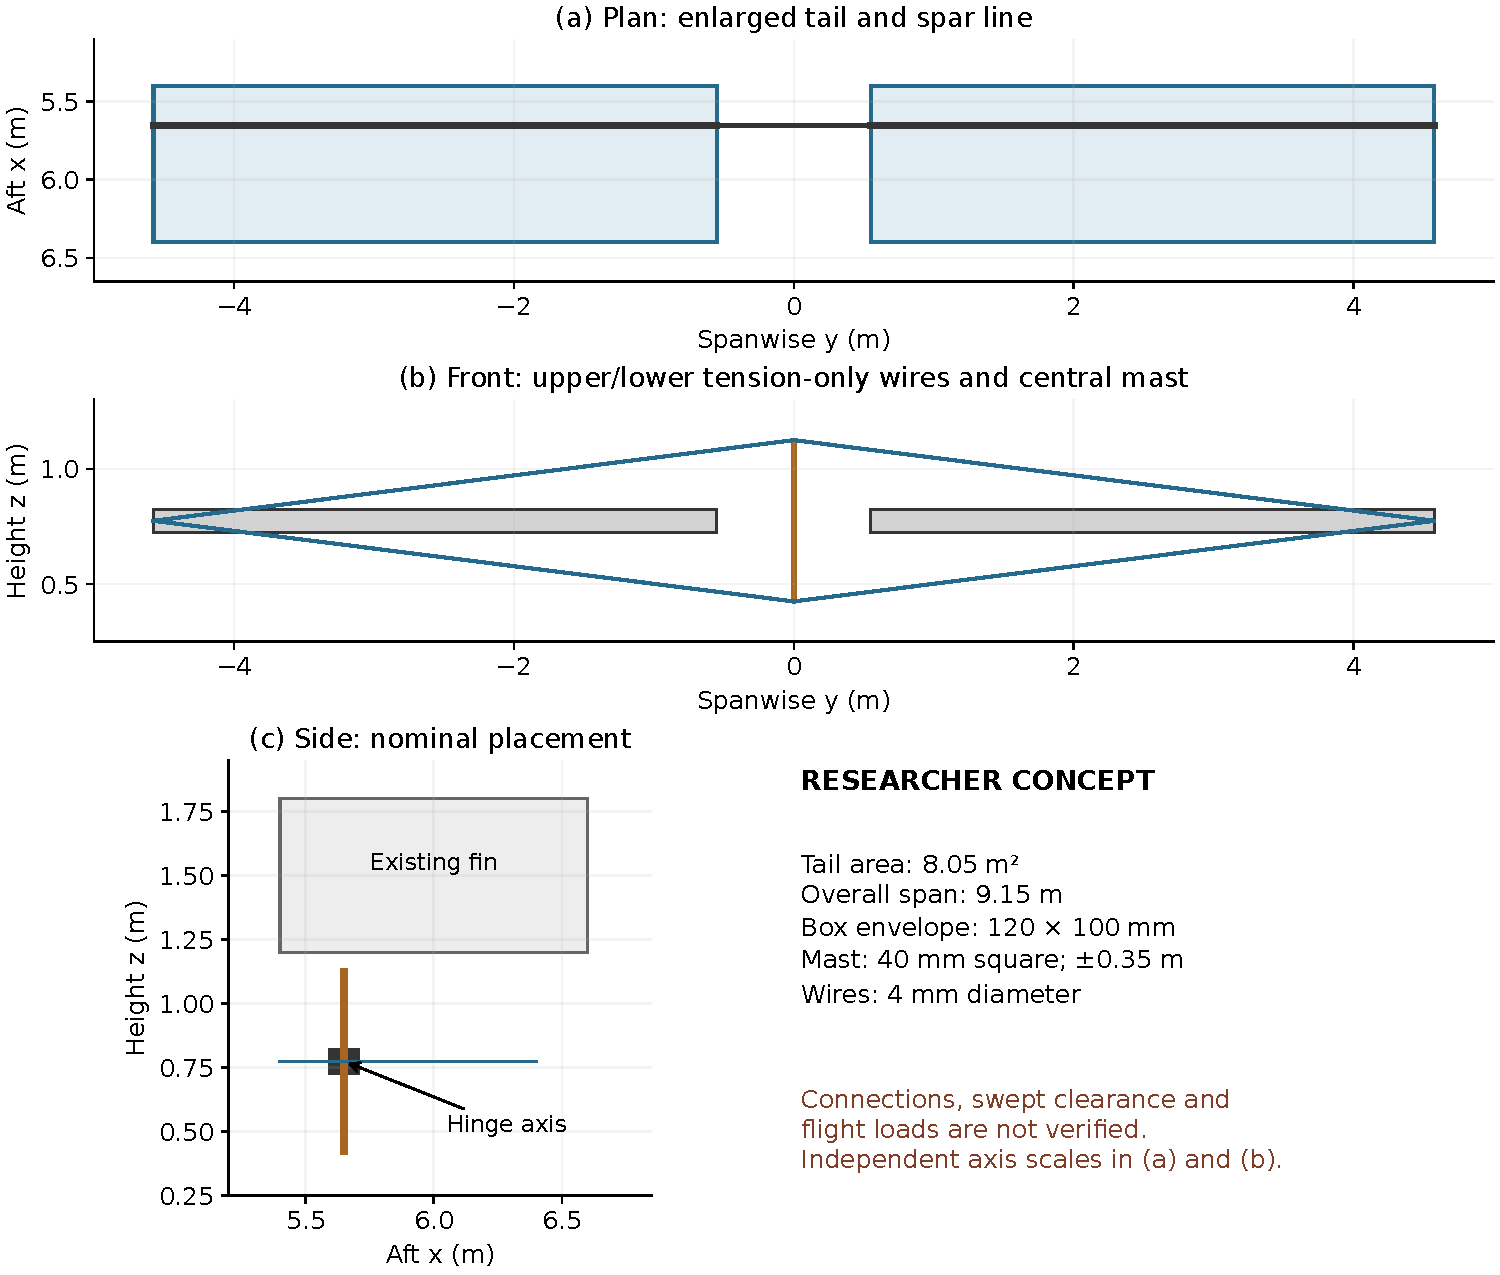
\includegraphics[width=\linewidth]{figures/braced_tail_concept.pdf}
\caption{Researcher braced-tail concept; connections remain unresolved.}
\label{fig:braced-tail-concept}
\end{figure}

The calculation couples a first-order bending beam to geometrically changing,
tension-only wires with zero initial prestress. Wire modulus 200 GPa and
density 7850 kg/m$^3$ are explicit evaluator assumptions, not identified or
certified wire properties. A wire is inactive when its computed extension
would place it in compression. At the evaluated downward load, the upper
wire is active and the lower wire is slack. The displacement compatibility
equation was solved without assigning compressive capacity to the slack wire.
The resulting tip displacement is 11.49 mm, compared with 39.80 mm for the
same box beam without bracing. The corresponding root moment is 139.21 N m
and upper-wire tension is 487.89 N. Multiplying the current strip loads and
weight by three gives 32.43 mm and 1417.29 N; this is only a load-scaling
exercise, not a derived 3-g flight load case. Beam-column effects, local
buckling, joint slip, load reversal, torsion and flutter remain outside the
model. Ideal Euler comparisons do not close those checks.

The calculated masses of the two boxes, four wires and mast are 6.116,
1.810 and 0.502 kg, respectively. Their sum, 8.429 kg, leaves 5.571 kg within
the earlier 14 kg tail allocation for ribs, covering, fittings, horns,
bearings and fasteners. That remainder is a mass budget, not a completed bill
of materials. The original assumed 14 kg ledger has therefore not been
replaced by a supposedly verified structural mass, and the earlier positive
static-margin prediction cannot be claimed for a fully integrated braced
airplane. This branch supplies explicit dimensions and testable requirements
for the next design iteration while retaining the failed additive-beam branch
as evidence of the coupled mass--stability problem.

